\documentclass[
	a4paper,
	oneside,
	DIV = 12,
	12pt,
	headings = normal,
]{scrartcl}

%%% Length calculations
\usepackage{calc}
%%%

%%% Support for color
\usepackage{xcolor}
\definecolor{lightblue}{HTML}{03A9F4}
\definecolor{red}{HTML}{F44336}
%%%

%%% Including graphics
\usepackage{graphicx}
%%%

%%% Font selection
\usepackage{fontspec}

\setromanfont{STIX Two Text}[
	SmallCapsFeatures = {LetterSpace = 5},
]

\setsansfont{IBM Plex Sans}[
	Scale = MatchUppercase,
]

\setmonofont{IBM Plex Mono}[
	Scale = MatchUppercase,
]
%%%

%%% Math typesetting
\usepackage{amsmath}

\usepackage{unicode-math}
\setmathfont{STIX Two Math}
%%%

%%% List settings
\usepackage{enumitem}
\setlist[enumerate]{
	label*      = {\arabic*.},
	leftmargin  = *,
	labelindent = \parindent,
	topsep      = 1\baselineskip,
	parsep      = 0\baselineskip,
	itemsep     = 1\baselineskip,
}

\setlist[itemize]{
	label*      = {—},
	leftmargin  = *,
	labelindent = \parindent,
	topsep      = 1\baselineskip,
	parsep      = 0\baselineskip,
	itemsep     = 1\baselineskip,
}

\setlist[description]{
	font        = {\rmfamily\upshape\bfseries},
	topsep      = 1\baselineskip,
	parsep      = 0\baselineskip,
	itemsep     = 0\baselineskip,
}

%%%

%%% Structural elements typesetting
\setkomafont{pagenumber}{\rmfamily}
\setkomafont{disposition}{\rmfamily\bfseries}

% Sectioning
\RedeclareSectionCommand[
	beforeskip = -1\baselineskip,
	afterskip  = 1\baselineskip,
	font       = {\normalsize\bfseries\scshape},
]{section}

\RedeclareSectionCommand[
	beforeskip = -1\baselineskip,
	afterskip  = 1\baselineskip,
	font       = {\normalsize\bfseries},
]{subsection}

\RedeclareSectionCommand[
	beforeskip = -1\baselineskip,
	afterskip  = 1\baselineskip,
	font       = {\normalsize\bfseries},
]{subsubsection}
%%%

%%% Typographic enhancements
\usepackage{microtype}
%%%

%%% Language-specific settings
\usepackage{polyglossia}
\setmainlanguage{ukrainian}
%%%

%%% Captions
\usepackage{caption}
\usepackage{subcaption}

%\DeclareCaptionLabelFormat{closing}{#2)}
%\captionsetup[subtable]{labelformat = closing}

%\captionsetup[subfigure]{labelformat = closing}

\captionsetup[table]{
	aboveskip = 0\baselineskip,
	belowskip = 1\baselineskip,
}

\captionsetup[figure]{
	aboveskip = 1\baselineskip,
	belowskip = 0\baselineskip,
}

\captionsetup[subfigure]{
	labelformat = simple,
	labelformat = brace,
}
%%%

%%% Table typesetting
\usepackage{booktabs}
\usepackage{longtable}

\usepackage{multirow}

\usepackage{array}
\newcolumntype{v}[1]{>{\raggedright\arraybackslash\hspace{0pt}}p{#1}}
\newcolumntype{b}[1]{>{\centering\arraybackslash\hspace{0pt}}p{#1}}
\newcolumntype{n}[1]{>{\raggedleft\arraybackslash\hspace{0pt}}p{#1}}
%%%

%%% Dingbats
\usepackage{pifont}
%%%

%%% Links and hyperreferences
\usepackage{hyperref}
\hypersetup{
	bookmarksnumbered = true,
	colorlinks      = false,
	linkbordercolor = red,
	urlbordercolor  = lightblue,
	pdfborderstyle  = {/S/U/W 1.5},
}
%%%

%%% Length adjustments
% Set baselineskip to ~15pt, default is 14.5pt
% \linespread{1.034483}
\linespread{1.068966} % ~15.5pt
\setlength{\emergencystretch}{1em}
\setlength{\parindent}{1.5em}
\newlength{\gridunitwidth}
\setlength{\gridunitwidth}{\textwidth / 12}
\setlength{\floatsep}{1\baselineskip}
\setlength{\intextsep}{1\baselineskip}
\setlength{\textfloatsep}{1\baselineskip}
%%%

%%% Custom commands
\newcommand{\allcaps}[1]{{\addfontfeatures{LetterSpace = 5}#1}}
\newcommand{\progname}[1]{\texttt{#1}}

\newcommand{\CheckMark}{\ding{51}}
%%%

\begin{document}
	\begin{titlepage}
		\begin{center}
			Міністерство освіти і науки України\\
			Національний авіаційний університет\\
			Навчально-науковий інститут комп'ютерних інформаційних технологій\\
			Кафедра комп'ютеризованих систем управління

			\vspace{\fill}
				Лабораторна робота №1.1\\
				з дисципліни «Діагностика та експлуатація комп'ютера»\\
				на тему «Встановлення операційної системи Windows XP на~віртуальну машину»\\

			\vspace{\fill}

			\begin{flushright}
				Виконав:\\
				студент \allcaps{ННІКІТ}\\
				групи СП-325\\
				Клокун В.\,Д.\\
				Перевів:\\
				Масловський Б.\,Г.
			\end{flushright}

			Київ 2018
		\end{center}
	\end{titlepage}

	\section{Ціль роботи}
		Ознайомлення з процесом встановлення операційної системи на віртуальну машину.

	\section{Короткі теоретичні відомості}
		Віртуальна машина~— це~програмна та/або~апаратна система, що~емулює апаратне забезпечення деякої платформи~(target~— цільова або~гостьова платформа) та~виконує програми для~target-платформи на~host-платформі~(host~— хост-платформа, платформа-хазяїн) або~віртуалізує деяку платформу та~створює на~ній середовища, які~ізолюють одне від~одної програми та~навіть операційні системи; також специфікація деякого обчислювального середовища (віртуальна машина~Java).

	\section{Хід роботи}
		Запускаємо програму VMware Player та~створюємо нову віртуальну машину, натиснувши на~кнопку~«Create a New Virtual Machine». У~з'я\-вив\-шо\-муся вікні створення віртуальної машини встановлюємо джерело встановлення на~шлях до~образу завантажувального диску з~системою Windows~XP і~натискаємо кнопку~«Next». У~наступному вікні заповнюємо дані аккаунту користувача для~розширення Easy~Install, натискаємо кнопку~«Next». У~новому вікні даємо віртуальній машині назву~«sp-325-klokun-rabin» і~натискаємо~«Next». У~вікні вибору розміру віртуального диску встановлюємо значення~20~Гб, натискаємо~«Next». У~з'явившомуся фінальному вікні перевіряємо налаштування віртуальної машини та~підтверджуємо їх, натискаючи кнопку~«Finish». 
		
		Підготувавши віртуальну машину до~роботи, запускаємо~її. Після запуску віртуальної машини починається процес встановлення операційної системи Windows~XP. Після завантаження установочних файлів обираємо автоматичний режим~— підсвічуємо опцію~«Automated Mode» та~натискаємо клавішу~Enter. Розпочинається первинний процес установки Windows~XP~(рис.~\ref{fig:01-winxp-install-primary}).
		\begin{figure}[!htbp]
			\centering
			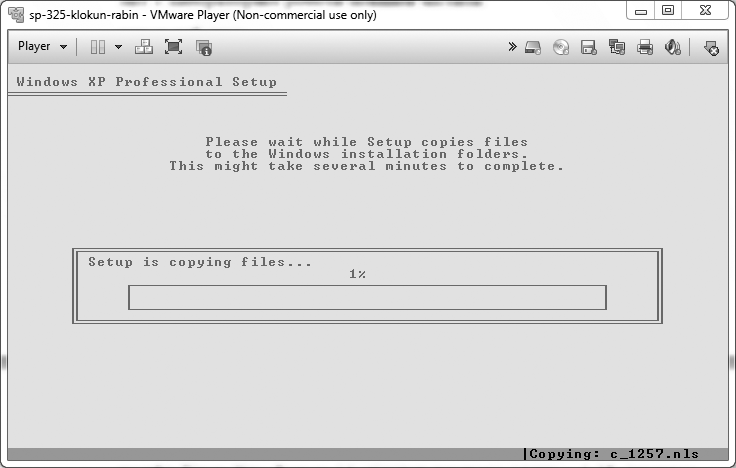
\includegraphics[height = 7\baselineskip]{./assets/y03s01-pcdiag-lab-01-01-bw.png}
			\caption{Початок первинного процесу установки Windows~XP}
			\label{fig:01-winxp-install-primary}
		\end{figure}

		Після закінчення первинної установки віртуальна машина перезавантажується та переходить до вторинного та фінального етапів, які повністю закінчують процес установки Windows~XP~(рис.~\ref{fig:02-winxp-install-secondary}).
		\begin{figure}[!htb]
			\centering
			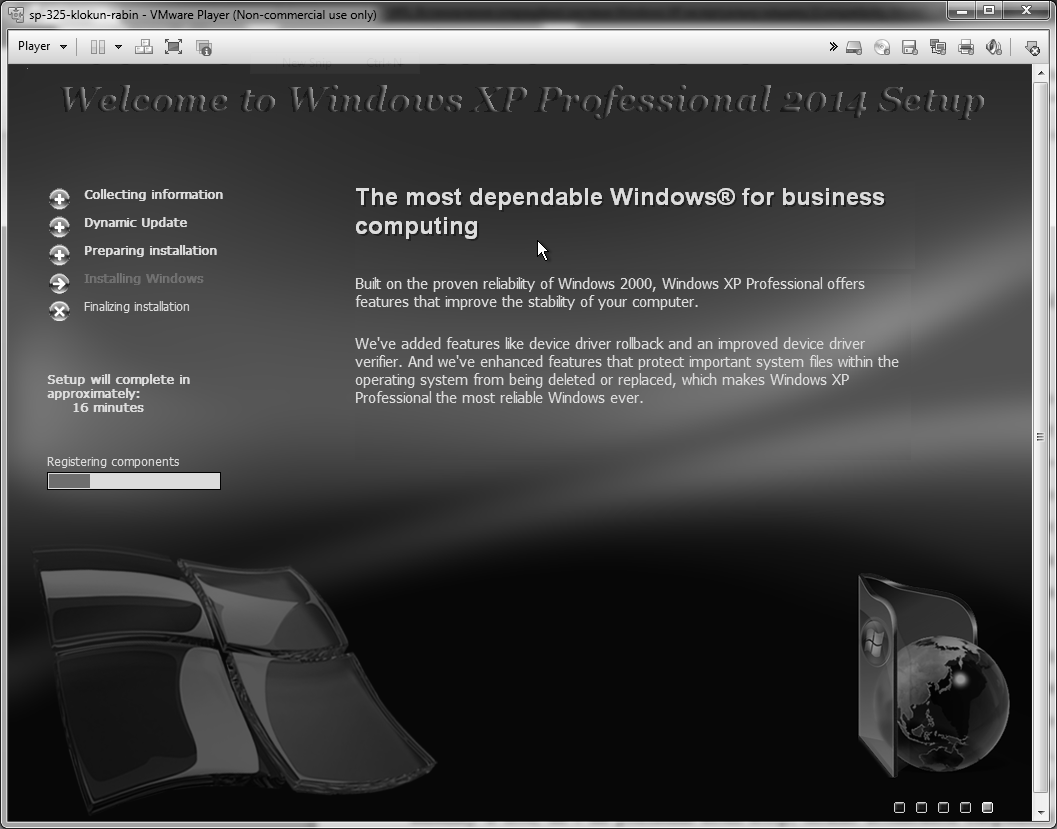
\includegraphics[height = 10\baselineskip]{./assets/y03s01-pcdiag-lab-01-02-bw.png}
			\caption{Вторинний етап установки Windows~XP}
			\label{fig:02-winxp-install-secondary}
		\end{figure}

		Після закінчення фінального етапу установки система виконує останні налаштування, готує аккаунт користувача та робочий стіл для нього і завантажується у робоче середовище~(рис.~\ref{fig:03-winxp-install-desktop}).
		\begin{figure}[!htb]
			\centering
			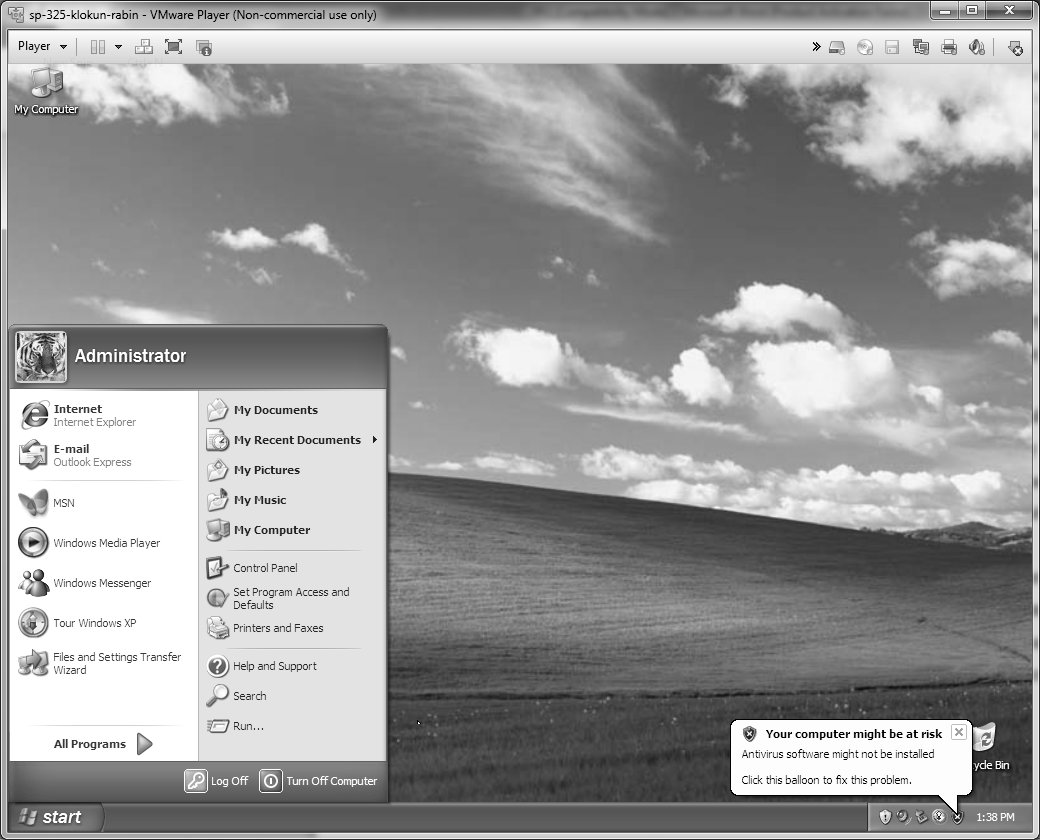
\includegraphics[height = 10\baselineskip]{./assets/y03s01-pcdiag-lab-01-03-bw.png}
			\caption{Результат установки Windows~XP}
			\label{fig:03-winxp-install-desktop}
		\end{figure}

	\section{Висновок}
		Виконуючи дану лабораторну роботу, ми~ознайомились з~процесом встановлення операційної системи на~віртуальну машину на~прикладі встановлення Microsoft Windows~XP на~віртуальну машину VMware~Player.

\end{document}
